\documentclass[journal]{IEEEtran}
\ifCLASSINFOpdf
\else
\fi
\hyphenation{op-tical net-works semi-conduc-tor}
\usepackage{booktabs}
\usepackage{float}
\usepackage{graphicx}
\usepackage{amsmath} 

\begin{document}
\title{Amplificadores basados en FET y circuitos de conmutación}
\author{Guido P. Krisdel Pamela, Gamboa Q. María José} 
\markboth{ITCR. Escuela de Ingeniería Electrónica. Laboratorio 8 – Amplificadores basados en JFET y circuitos de conmutación}
{Shell \MakeLowercase{\textit{et al.}}: Bare Demo of IEEEtran.cls for IEEE Journals}

\maketitle
\renewcommand{\abstractname}{Resumen}
\begin{abstract}
En este informe se estudia el comportamiento de amplificadores con transistores JFET, específicamente en configuraciones de fuente común y drenador común. Se construyeron y analizaron ambos circuitos, evaluando sus parámetros en corriente continua (DC) y corriente alterna (CA), incluyendo ganancia de tensión, desfase entre señales de entrada y salida, y la respuesta ante fallas comunes. Además, se observó el efecto de la variación en la resistencia de carga y el uso de una fuente de corriente en la mejora de la ganancia del amplificador. Los resultados permiten comprender el funcionamiento, limitaciones y ventajas de estas configuraciones en aplicaciones electrónicas donde se requiere amplificación de señales pequeñas.
\end{abstract}

\renewcommand{\IEEEkeywordsname}{Palabras clave}
\begin{IEEEkeywords}
amplificador JFET, fuente común, drenador común, ganancia de tensión
\end{IEEEkeywords}

\IEEEpeerreviewmaketitle

\section{Introduction}
\IEEEPARstart{L}{os}
amplificadores utilizando transistores JFET son fundamentales en el diseño de circuitos electrónicos debido a su alta impedancia de entrada y bajo consumo de potencia. Entre las configuraciones más comunes se encuentran el amplificador en fuente común y el amplificador en drenador común, cada uno con características particulares que afectan el comportamiento de la señal amplificada.
\par El objetivo principal del experimento fue analizar el comportamiento de estas configuraciones ante distintas condiciones de operación, midiendo parámetros tanto en corriente continua como en corriente alterna. Se estudió la respuesta del circuito ante cambios en la resistencia de carga, así como los efectos de polarización mediante una fuente de corriente. Además, se evaluó la ganancia de tensión, la diferencia de fase entre la señal de entrada y salida, y la respuesta del circuito ante fallas específicas.
\par A partir del análisis experimental, se concluye que la elección de la configuración y polarización del JFET influye directamente en el rendimiento del amplificador. Esta comprensión es esencial para el diseño de sistemas que requieren amplificación precisa y eficiente de señales en aplicaciones electrónicas variadas.

\section{MATERIALES Y EQUIPO}
Para la realización de ambas configuraciones del experimento se emplearon los siguientes equipos de medición:
\begin{itemize}
    \item 1 Generador de señales
    \item 1 Osciloscopio
    \item 1 Multímetro
\end{itemize}
\par Para la configuración del amplificador en fuente común se empleó los siguientes componentes electrónicos:
\begin{itemize}
    \item 1 Resistencia de 56 $\Omega$
    \item 1 Resistencia de 6.8k $\Omega$
    \item 1 Resistencia de 10k $\Omega$
    \item 1 Resistencia de 100k $\Omega$
    \item 1 Resistencia de 10M $\Omega$
    \item 1 Capacitor de 0.1$\mu$ F
    \item 1 Capacitor de 1$\mu$ F
    \item 1 Capacitor de 10$\mu$ F
    \item 1 Transistor JFET 2N5458 
\end{itemize}
\par Para la configuración del amplificador en drenador común se empleó los siguientes componentes electrónicos:
\begin{itemize}
    \item 1 Resistencia de 100 $\Omega$
    \item 1 Resistencia de 1k $\Omega$
    \item 1 Resistencia de 10k $\Omega$
    \item 1 Resistencia de 100k $\Omega$
    \item 1 Resistencia de 220 $\Omega$
    \item 1 Resistencia de 1M $\Omega$
    \item 1 Capacitor de 0.1$\mu$ F
    \item 1 Capacitor de 10$\mu$ F
    \item 1 Potenciómetro de 500 $\Omega$
    \item 2 Transistores JFET 2N5458
\end{itemize}

\section{Resultados Experimentales}
\textbf{Amplificador en drenador común}
\par Se presentan los datos obtenidos durante la ejecución del experimento en la parte correspondiente al amplificador con drenador común. Se incluyen mediciones realizadas con los instrumentos de laboratorio, así como observaciones relevantes sobre el comportamiento del circuito. Además, se comparan los resultados experimentales con los valores teóricos y simulaciones para analizar la precisión de las mediciones.
\par Para garantizar la precisión de los resultados obtenidos en el experimento, se realizó una medición previa de los valores de las resistencias y capacitores, y así, asegurar que los valores reales estuvieran dentro de la tolerancia especifica. Los valores obtenidos en la medición se presentan en la siguiente tabla:
\begin{table}[h]
    \caption{Comparación entre valores teóricos y experimentales de resistencias.}
    \centering
    \renewcommand{\arraystretch}{1.2} % Ajusta la altura de las filas
    \begin{tabular}{|l|p{2cm}|p{2cm}|p{2cm}|}
        \hline
        & \textbf{Valor Teórico [$\Omega$]} & \textbf{Valor Experimental [$\Omega$]} & \textbf{Porcentaje de error [\%]} \\
        \hline
        R1 & 100  & 101.003  & 1 \\
        \hline
        R2 & 1k   & 0.997k  & 0.30 \\
        \hline
        R3 & 10k & 9.909k & 0.91 \\
        \hline
        R3 & 220 & 220.672 & 0.30 \\
        \hline
        R3 & 1M & 0.986M & 1.4 \\
        \hline
    \end{tabular}
    \label{tab:resistencias}
\end{table}
\par A partir de los datos obtenidos, se evidencia que los valores experimentales de las resistencias presentan una buena concordancia con los valores teóricos. El porcentaje de error registrado en cada caso se mantiene igual o por debajo de 1.4, lo cual es coherente con las tolerancias esperadas en componentes electrónicos de uso general. Estos resultados permiten asegurar que los componentes empleados son adecuados para el desarrollo experimental y garantizan mediciones confiables.
\par Se procedió con la construcción del circuito amplificador en drenador común, según lo ilustrado en la Figura 1. 
\begin{figure}[H]
    \centering
    \includegraphics[width=0.5\textwidth]{Media/amplificador_drenador_común.png}
    \caption{Amplificador en drenador común.}
    \label{fig:amplificador_drenador_común.}
\end{figure}
\par Una vez ensamblado el circuito, se midieron las tensiones en corriente directa (CD) en los terminales de drenador, fuente y compuerta del transistor JFET. A partir de la tensión medida en la resistencia \( R_S \), se calculó la corriente \( I_D \) correspondiente. Todos los valores obtenidos fueron registrados en la Tabla 2 para su análisis comparativo.
\begin{table}[h]
    \caption{Comparación parámetros CD para el amplificador en drenador común}
    \centering
    \renewcommand{\arraystretch}{1.2} % Ajusta la altura de las filas
    \begin{tabular}{|l|p{2cm}|p{2cm}|p{2cm}|}
        \hline
        & \textbf{Valor Teórico} & \textbf{Valor Experimental} & \textbf{Porcentaje de error [\%]} \\
        \hline
        \( V_G \) & 0 V  & 0.054m V  & 0.05 \\
        \hline
        \( V_S \) & 209.402m V   & 210.121m V  & 0.34 \\
        \hline
        \( V_D \) & 15 V & 15.011 V & 0.07 \\
        \hline
        \( I_D \) & 269, 847m A & 268.672m A & 0.43 \\
        \hline
    \end{tabular}
    \label{tab:resistencias}
\end{table}
\par En la comparación de los parámetros del amplificador en drenador común, se observa que los valores experimentales obtenidos están muy cerca de los valores teóricos, lo que indica una buena concordancia entre ambos. El porcentaje de error se mantiene bajo en todos los casos, con el valor más bajo registrado en \( V_G \), y el más alto en \( I_D \). En general, los errores porcentuales son mínimos, lo que refleja una correcta implementación del amplificador en drenador común.
\par Posteriormente, se utilizaron las puntas del osciloscopio para observar simultáneamente la señal de entrada y la señal de salida en corriente alterna (CA), con el fin de analizar su comportamiento dinámico, según lo ilustrado en la Figura 2. 
\begin{figure}[H]
    \centering
    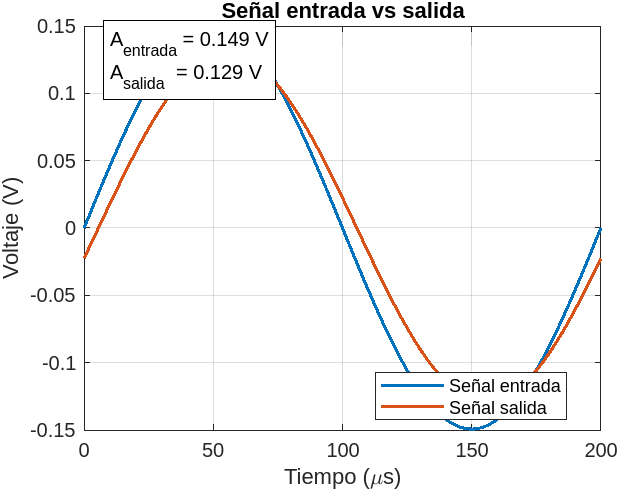
\includegraphics[width=0.5\textwidth]{Media/onda_entrada_salida.png}
    \caption{Onda entrada vs salida.}
    \label{fig:onda_entrada_salida.}
\end{figure}
\par Se determinó el desfase entre ambas señales y se calculó la ganancia de tensión del amplificador. Todos los valores obtenidos fueron registrados en la Tabla 3 para su análisis comparativo.
\begin{table}[h]
    \caption{Comparación parámetros CA para el amplificador en drenador común}
    \centering
    \renewcommand{\arraystretch}{1.2} % Ajusta la altura de las filas
    \begin{tabular}{|l|p{2cm}|p{2cm}|p{2cm}|}
        \hline
        & \textbf{Valor Teórico} & \textbf{Valor Experimental} & \textbf{Porcentaje de error [\%]} \\
        \hline
        \( V_{ent}\) & 149.268m V   & 150m V  & 0.49 \\
        \hline
        \( V_{SAL} \) & 129.198m V    & 126m V  & 2.47 \\
        \hline
        \( A_V \) & 0.865 & 0.840 & 2.89 \\
        \hline
        Desfase & $0^\circ$ & $0^\circ$ & 0 \\
        \hline
    \end{tabular}
    \label{tab:resistencias}
\end{table}
\par En la comparación de los parámetros de corriente alterna (CA) para el amplificador en drenador común, se observa que los valores experimentales están en cercanía con los valores teóricos. El porcentaje de error es bajo en general, destacando el valor de \( V_{ent}\) con un error de 0.49, mientras que el valor más alto corresponde a \( V_{SAL} \) con un error de 2.47. El factor de amplificación \( A_V \) presenta un error de 2.89, lo que es también un valor relativamente bajo. Además, el desfase entre las señales es nulo, coincidiendo con el valor teórico de $0^\circ$. Estos resultados indican que el comportamiento del amplificador en drenador común es consistente con las expectativas teóricas en cuanto a su desempeño en corriente alterna.
\par Seguidamente, se aumentó progresivamente la amplitud de la señal de entrada\( V_S \) con el fin de observar el comportamiento del amplificador ante señales de mayor exigencia. Se encontró que con una amplitud de 255m\( V_P \), la salida se mantenía sin distorsión visible. No obstante, a partir de 265m\( V_P \) comenzaron a notarse ligeras alteraciones en la forma de onda, que se hicieron más evidentes en 270m\( V_P \), y finalmente se observó un recorte claro en 300m\( V_P \).
\par En ese punto, la señal de salida alcanzó un valor máximo de 262.6913m\( V_P \) y un valor mínimo de -190.835m\( V_P \), evidenciando que el amplificador dejó de operar dentro de su región lineal. Este comportamiento se debe a que el transistor JFET alcanza sus límites de conducción: al aumentar demasiado la amplitud de la señal de entrada, el transistor entra en saturación o corte, impidiendo que la señal de salida reproduzca fielmente la forma de la señal de entrada [1].
\par A partir del circuito desarrollado en el experimento anterior, se realizó una modificación que consistió en agregar una fuente de corriente con el fin de mejorar la ganancia de tensión del amplificador en configuración de drenador común, según se ilustra en la Figura 3.
\begin{figure}[H]
    \centering
    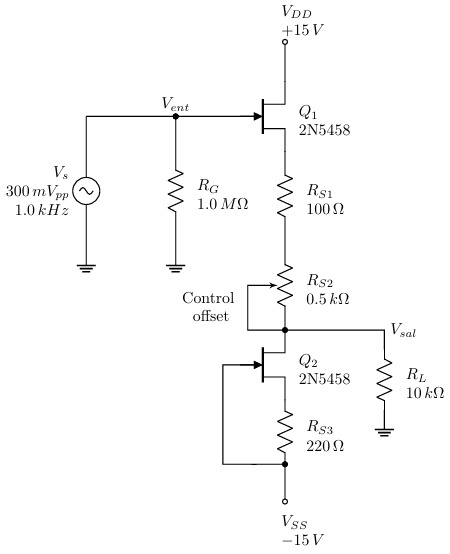
\includegraphics[width=0.5\textwidth]{Media/amplificador_fuente_corriente.png}
    \caption{Amplificador en drenador común con fuente de corriente.}
    \label{fig:amplificador_fuente_corriente.}
\end{figure}
\par Esta etapa del experimento permite observar cómo la incorporación de un JFET adicional, actuando como fuente de corriente, influye directamente en el comportamiento del sistema. La ganancia de tensión en este tipo de configuración es típicamente menor a uno, debido a la transconductancia $g_m$, que puede modelarse como una resistencia interna equivalente a $\frac{1}{g_m}$. Dicha resistencia se comporta de forma análoga al $r'_e$ de un transistor bipolar, aunque es mayor para una misma corriente, y junto con $R_S$, forma un divisor de tensión que limita la ganancia [1].
\par Para contrarrestar este efecto, se implementó una fuente de corriente con un JFET, ilustrado en la Figura 4, aprovechando su alta resistencia interna. Esta configuración eliminó los capacitores de acople, lo cual representa una ventaja para la respuesta en frecuencias bajas. Además, se sustituyó el resistor de la fuente por un potenciómetro que permitió ajustar el nivel de corriente continua (DC) en la señal de salida [1]. En este diseño, la salida se tomó desde el drenador del transistor $Q_2$, que cumple la función de fuente de corriente, mientras que el transistor $Q_1$ sigue operando como amplificador en configuración de drenador común.
\par El osciloscopio se colocó en modo de acoplamiento DC para observar la señal de salida, y se ajustó el potenciómetro $R_{S2}$ hasta obtener el menor offset posible en $V_{\text{sal}}$. Se ajusta $R_{S2}$ a 150~$\Omega$, quedando como valor máximo en 123.369mV y valor mínimo en -164.875~mV. Luego, se midieron y registraron los parámetros de tensión tanto en corriente continua como en alterna, los cuales se consignaron en la Tabla 4 y Tabla 5. 
\begin{table}[h]
    \caption{Comparación parámetros CD para el amplificador en drenador común con fuente de corriente}
    \centering
    \renewcommand{\arraystretch}{1.2} % Ajusta la altura de las filas
    \begin{tabular}{|l|p{2cm}|p{2cm}|p{2cm}|}
        \hline
        & \textbf{Valor Teórico} & \textbf{Valor Experimental} & \textbf{Porcentaje de error [\%]} \\
        \hline
        \( V_{G(Q1)} \) & 0 V  & 0.054m V  & 0.05 \\
        \hline
        \( V_{S(Q1)} \) & 157.632m V   & 156.921m V  & 0.45 \\
        \hline
        \( V_{D(Q1)} \) & 15 V & 15.011 V & 0.07 \\
        \hline
        \( V_{G(Q2)} \) & -15 V  & -15.011 V  & 0.07 \\
        \hline
        \( V_{S(Q2)} \) & -14.843 V   & -14.586 V  & 1.73 \\
        \hline
        \( V_{D(Q2)} \) & -20.7m V & -20.929 V & 1.1 \\
        \hline
        \( I_D \) & 1.5m A & 1.487m A & 0.86 \\
        \hline
    \end{tabular}
    \label{tab:resistencias}
\end{table}
\begin{table}[h]
    \caption{Comparación parámetros CA para el amplificador en drenador común con fuente de corriente}
    \centering
    \renewcommand{\arraystretch}{1.2} % Ajusta la altura de las filas
    \begin{tabular}{|l|p{2cm}|p{2cm}|p{2cm}|}
        \hline
        & \textbf{Valor Teórico} & \textbf{Valor Experimental} & \textbf{Porcentaje de error [\%]} \\
        \hline
        \( V_{ENT} \) & 149.725m V  & 150m V  & 0.18 \\
        \hline
        \( V_{SAL} \) & 123.369m V   & 125.432m V  & 1.67 \\
        \hline
        \( A_V \) & 0.823 & 0.836 & 1.57 \\
        \hline
        Desfase & $0^\circ$  & $0^\circ$  & 0 \\
        \hline
    \end{tabular}
    \label{tab:resistencias}
\end{table}
\par A partir del análisis de las Tablas correspondientes a los parámetros en corriente directa (CD) y corriente alterna (CA) para el amplificador en drenador común polarizado con una fuente de corriente, se evidencia un alto grado de precisión entre los valores teóricos y los experimentales. En los parámetros CD, los voltajes medidos en compuerta, fuente y drenador de ambos transistores presentaron errores mínimos, generalmente inferiores al 0.1\,\%, lo cual refleja un montaje adecuado y un correcto funcionamiento del circuito. En cuanto a la corriente de drenaje (\( I_D \)), su valor experimental se mantuvo cercano al teórico, indicando que la polarización fue estable y coherente con el diseño esperado.
\par Respecto a los parámetros CA, la señal de entrada (\( V_{ENT} \)) y la de salida (\( V_{SAL} \)) mostraron una relación coherente, permitiendo calcular una ganancia en tensión (\( A_V \)) aproximada de 0.83, valor que valida el comportamiento esperado del amplificador en esta configuración. Además, no se observó desfase entre ambas señales, lo cual es característico del amplificador en drenador común. En general, las mediciones respaldan el correcto desempeño del circuito, y la inclusión de una fuente de corriente permitió mejorar la ganancia manteniendo una buena estabilidad de la señal.
\par En esta sección del experimento se procedió a analizar el comportamiento del amplificador en drenador común con fuente de corriente ante señales de entrada con amplitudes crecientes, con el fin de identificar el punto de recorte o saturación de la señal de salida. Se incrementó progresivamente la amplitud de la señal de entrada (\( V_S \)), comenzando con valores bajos para observar el comportamiento lineal del sistema. Se observó que, con una amplitud de 6(\( V_P \)), la salida permanecía sin distorsión visible; sin embargo, al aumentar a 7(\( V_P \)), comenzaron a percibirse ligeras deformaciones en la forma de onda. Estas alteraciones se hicieron más notorias a 8(\( V_P \)) y resultaron claramente visibles a 10(\( V_P \)), momento en el cual se presentó un recorte evidente en la señal de salida.
\par En este punto de saturación, la salida alcanzó un valor máximo de 7.744 V y un mínimo de -6.414 V, lo que indica que el amplificador salió de su región lineal de operación. Este recorte se debe a que el transistor JFET llega a sus límites de conducción, entrando en saturación o corte, y por lo tanto no puede seguir reproduciendo fielmente la forma de la señal de entrada [1]. Esta observación evidencia la importancia de mantener la entrada dentro del rango dinámico permitido para evitar distorsiones significativas.
\par La ganancia del amplificador mejoró considerablemente al sustituir la resistencia de fuente (\( R_S \)) por una fuente de corriente activa con JFET. Aunque los valores numéricos de ganancia obtenidos fueron cercanos 0.8655 para la configuración con autopolarización y 0.8239 para la configuración con fuente de corriente, el cambio en la estructura del circuito trajo consigo mejoras en el comportamiento general de la señal. Este comportamiento indica que, aunque la ganancia en valores absolutos se redujo ligeramente, la fuente de corriente permite un mayor rango dinámico y una menor distorsión bajo señales exigentes [1], lo cual representa una mejora real en el desempeño del amplificador.
\newline
\\
\textbf{Amplificador en fuente común}

\section{Conclusion}
\par En el amplificador en drenador común sin la incorporación de una fuente de corriente, se observó una ganancia de tensión menor a la unidad, lo cual es característico de esta configuración debido a la presencia de una resistencia interna del transistor ($\frac{1}{g_m}$) que, junto con la resistencia de fuente $R_S$, forma un divisor de tensión. Esta limitación en la ganancia refleja la naturaleza amortiguada del circuito, siendo útil en aplicaciones como buffers, pero ineficiente si se requiere amplificación significativa de señal.
\par Al implementar una fuente de corriente mediante un segundo transistor JFET ($Q_2$), se logró una mejora notable en la ganancia del amplificador en drenador común. Esto se debe a la alta resistencia de salida ofrecida por la fuente de corriente, que minimiza el efecto divisor de tensión entre $R_S$ y $\frac{1}{g_m}$, permitiendo que una mayor proporción de la señal se transmita a la salida. Además, la eliminación de capacitores de acople favorece una mejor respuesta en bajas frecuencias, haciendo esta configuración más eficiente y versátil para aplicaciones que requieren una mayor fidelidad en la amplificación de señales.


\appendices
\section{}
\noindent\textbf{Ganancia de tensión ($A_v$)}
\par La ganancia de tensión de un amplificador en drenador común se define como la relación entre la señal de salida y la señal de entrada [1]:
\begin{equation}
A_v = \frac{V_{SAL}}{V_{ENT}}
\end{equation}
\par Donde:
\begin{itemize}
    \item $V_{SAL}$ es la amplitud pico a pico de la señal de salida.
    \item $V_{ENT}$ es la amplitud pico a pico de la señal de entrada.
\end{itemize}
\par En esta configuración, dado que el circuito actúa como un seguidor de fuente, la ganancia típica es ligeramente menor a 1 debido a la resistencia interna del transistor [1]:
\begin{equation}
A_v \approx \frac{g_m R_L}{1 + g_m R_S}
\end{equation}
\par Donde:
\begin{itemize}
    \item $g_m$ es la transconductancia del JFET.
    \item $R_L$ es la carga conectada en la salida (normalmente igual a $R_L$ externo o equivalente).
    \item $R_S$ es la resistencia de fuente.
\end{itemize}
\\
\newline
\textbf{Diferencia de fase entre señales}
\par La diferencia de fase entre la señal de entrada y la salida puede observarse utilizando un osciloscopio en modo XY o superponiendo ambas señales en modo tiempo. En el caso del amplificador en drenador común, la salida está prácticamente en fase con la entrada, aunque puede haber un ligero retardo de fase debido a las capacidades parásitas [1].
\par Para calcular la diferencia de fase ($\phi$) se puede usar:
\begin{equation}
\phi = \frac{\Delta t}{T} \times 360^\circ
\end{equation}
\par Donde:
\begin{itemize}
    \item $\Delta t$ es la diferencia de tiempo entre los picos (o cruces por cero) de las señales de entrada y salida.
    \item $T$ es el período de la señal.
\end{itemize}
\par La diferencia de fase se mide en grados ($^\circ$), y un desfase positivo indica que la salida va retrasada con respecto a la entrada.
\\
\newline
\textbf{Interpretación de diferencia de fase entre señales}
\subsubsection*{Desfase de 0°}
\par Cuando se dice que hay un desfase de 0°, significa que la señal de salida está en fase con la señal de entrada. Es decir, ambas señales alcanzan sus valores máximos, mínimos y puntos de cruce por cero al mismo tiempo [1]. Esto es típico en configuraciones como el amplificador en drenador común (seguidor de fuente).
\begin{itemize}
    \item La forma de onda de salida es prácticamente una copia atenuada de la entrada.
    \item No hay inversión de señal.
\end{itemize}
\subsubsection*{Desfase de 180°}
\par Un desfase de 180° indica que la señal de salida está invertida respecto a la entrada. Cuando la entrada está en su punto máximo, la salida está en su punto mínimo, y viceversa [1].
\begin{itemize}
    \item Es característico de configuraciones como el amplificador en fuente común.
    \item La salida es una imagen especular (invertida verticalmente) de la entrada.
\end{itemize}
\ifCLASSOPTIONcaptionsoff
  \newpage
\fi

\begin{thebibliography}{1}
\bibitem{alexander}
C. K. Alexander and M. N. O. Sadiku, \textit{Fundamentos de circuitos eléctricos}. México ; Madrid Etc.: McGraw-Hill, 2018.
\end{thebibliography}
\end{document}



